
%(BEGIN_QUESTION)
% Copyright 2006, Tony R. Kuphaldt, released under the Creative Commons Attribution License (v 1.0)
% This means you may do almost anything with this work of mine, so long as you give me proper credit

Complete the truth table for the following relay logic circuit, and then complete a second truth table for the same circuit with relay coil CR2 failed open:

$$\includegraphics[width=15.5cm]{i02318x01.eps}$$

Assume a ``1'' state for a switch means it is being pressed, and a ``0'' state means it is unpressed.  Explain {\it why} the truth table will be modified as a result of the fault.

\vskip 20pt \vbox{\hrule \hbox{\strut \vrule{} {\bf Suggestions for Socratic discussion} \vrule} \hrule}

\begin{itemize}
\item{} Identify how ladder-logic type diagrams differ from standard electronic schematics, particularly with regard to how electromechanical relay coils and contacts are shown in each.
\item{} Suppose the indicator lamp in this circuit {\it never} energized, regardless of the switch states.  Identify soe possible faults that could account for this circuit behavior, and how you could confirm those faults using a multimeter.
\end{itemize}

\underbar{file i02318}
%(END_QUESTION)





%(BEGIN_ANSWER)

$$\includegraphics[width=15.5cm]{i02318x02.eps}$$

If you thought that the ``faulted'' truth table would be all 0's, you probably thought I said relay {\it contact} CR2 failed open.  The fault I proposed was relay CR2 {\bf coil} failed open.

%(END_ANSWER)





%(BEGIN_NOTES)

The purpose of this question is to approach the domain of circuit troubleshooting from a perspective of knowing what the fault is, rather than only knowing what the symptoms are.  Although this is not necessarily a realistic perspective, it helps students build the foundational knowledge necessary to diagnose a faulted circuit from empirical data.  Questions such as this should be followed (eventually) by other questions asking students to identify likely faults based on measurements.

\vfil \eject

\noindent
{\bf Summary Quiz:}

Identify one component fault in this relay circuit that would {\it not} cause the indicator lamp to always remain off (unlit):

$$\includegraphics[width=15.5cm]{i02318x03.eps}$$

\begin{itemize}
\item{} Relay contact CR1 failed open
\vskip 5pt 
\item{} Relay coil CR2 failed open
\vskip 5pt 
\item{} Switch contact A failed open
\vskip 5pt 
\item{} Relay contact CR2 failed open
\vskip 5pt 
\item{} Switch contact B failed shorted
\vskip 5pt 
\item{} Relay coil CR1 failed open
\end{itemize}


%INDEX% Relay, diagram: ladder logic

%(END_NOTES)


